\documentclass[a4paper,10pt]{article}
\usepackage[T1]{fontenc}
\usepackage[utf8]{inputenc}
\usepackage[english]{babel}
\usepackage{lmodern}
\usepackage[top=1.3cm,bottom=1.4cm,left=1.6cm,right=1.6cm]{geometry}
\usepackage{titlesec,enumitem,xcolor,graphicx,lastpage,fancyhdr}
\usepackage{fontawesome5}
\usepackage[hidelinks]{hyperref}

\hypersetup{colorlinks=true,urlcolor=blue!70!black,linkcolor=blue!70!black}
\pagestyle{fancy}\fancyhf{}\renewcommand{\headrulewidth}{0pt}
\fancyfoot[C]{\small\color{gray}Page \thepage\ of \pageref{LastPage}}
\setlength{\parindent}{0pt}

\titleformat{\section}{\large\bfseries\color{blue!70!black}}{}{0em}{}[\vspace{-0.7em}\rule{\textwidth}{0.5pt}]
\titlespacing{\section}{0pt}{6pt}{3pt}
\setlist[itemize]{leftmargin=1.1em,itemsep=2pt,topsep=2pt,parsep=0pt}
\newcommand{\role}[4]{\vspace{3pt}\noindent\hspace{0.6em}\parbox[t]{0.38\textwidth}{\raggedright\textbf{#1}}\hfill\parbox[t]{0.58\textwidth}{\raggedleft\textit{#2}}\\{\textit{#3}\hfill\textit{#4}}\vspace{1pt}}

\begin{document}
\noindent
\begin{minipage}[t]{0.78\textwidth}
\vspace{0pt}
{\huge\bfseries Prabhavit Gupta}\\[8pt]
{\small \faPhone\ +39-351-610-7807 \quad \faEnvelope\ \href{mailto:prabhavitg@gmail.com}{prabhavitg@gmail.com} \quad \faLinkedin\ \href{https://www.linkedin.com/in/prabhavit/}{Linkedin} \quad \faMapMarker*\ Venice, Italy}
\end{minipage}\hfill
\begin{minipage}[t]{0.18\textwidth}
\vspace{0pt}\raggedleft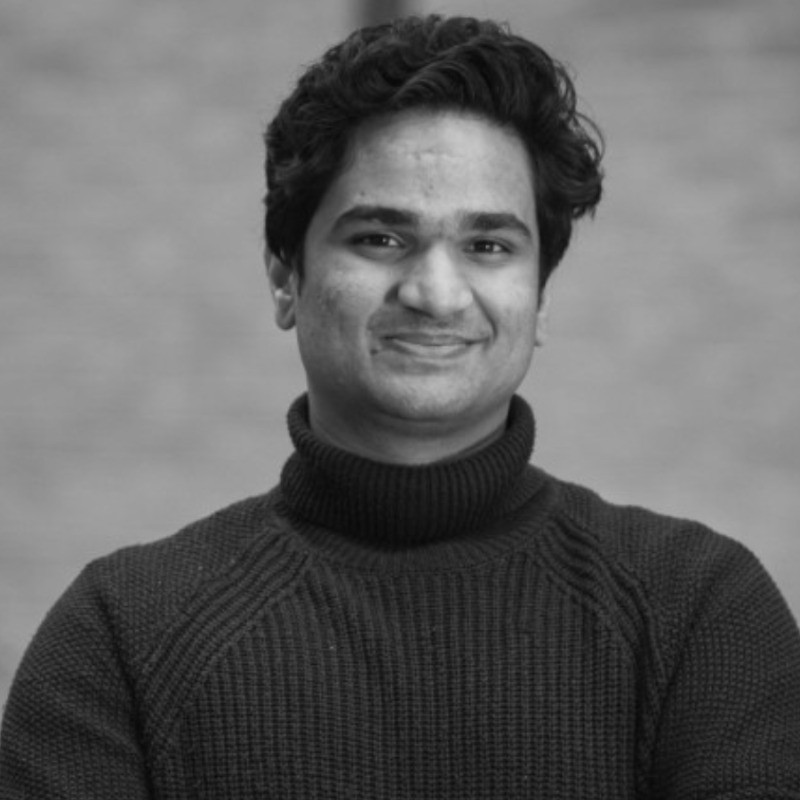
\includegraphics[width=2.3cm,height=2.3cm,keepaspectratio]{photo.jpg}
\end{minipage}

\section{Career Summary}
\begin{itemize}
\item Automation and software integration engineer with hands-on experience in sensor data acquisition, telemetry pipelines, and Linux runtime environments.
\item Proficient in Python scripting, API protocols, containerized testing (Docker), and automated quality validation workflows.
\item Experienced in hardware device interfacing, technical documentation, and rigorous root-cause troubleshooting for production deployments.
\end{itemize}

\section{Technical Skills}
\begin{itemize}
\item \textbf{Automation \& Systems} -- Python, C++ Fundamentals, Shell Scripting (Bash), Linux OS, Git Flow, CI/CD, Containerization (Docker)
\item \textbf{Sensor Integration \& Telemetry} -- Hardware Interfacing, Device Telemetry, REST APIs, Webhooks, Data Pipeline Processing
\item \textbf{AI \& Intelligent Workflows} -- Edge AI Integration, Structured Data Extraction, Computer Vision API Integration, Model Telemetry
\item \textbf{Testing \& Quality Assurance} -- Automated Regression Testing, Unit Testing, QA Validation, Root Cause Analysis, Runbook Authoring
\end{itemize}

\section{Visa \& Language}
\begin{itemize}
\item \textbf{Language} -- English (Fluent / Professional), Italian (Conversational / Intermediate), Hindi (Native)
\item \textbf{Work Authorization} -- European Long Term Residence Permit (Italy, no sponsorship needed). Available immediately.
\end{itemize}

\section{Professional Experience}
\role{\href{https://flowspace.co}{FlowSpace.co}}{Systems Automation \& Software Developer (Full time, Freelance)}{London, UK / Remote}{Mar 2024 -- Ongoing}
\begin{itemize}
\item \textbf{Product Responsibilities:}
\begin{itemize}[label=--]
\item Supported platform scaling to over 4,500 active users through continuous integration cycles and system performance monitoring.
\item Oversaw platform migration off a legacy stack to a modern Next.js and backend service architecture, guaranteeing zero downtime.
\item Documented operational system logic, service dependencies, and error handling mechanisms across development teams.
\item Integrated AI agent services to automate diagnostic ticket sorting and routine operational queries.
\end{itemize}
\item \textit{Tools: Python, Docker, Linux, Git, Jira, Postman}
\item \textbf{Technical Responsibilities:}
\begin{itemize}[label=--]
\item Developed Python utilities and n8n pipelines for automated data extraction, parsing, and structured database synchronization.
\item Configured webhook endpoints and REST interfaces to synchronize distributed event streams across external service providers.
\item Performed end-to-end integration validation and automated smoke testing across staging and production environments.
\item \textit{Tools: Python, Bash, REST APIs, n8n, Git, Postman, Docker}
\end{itemize}
\end{itemize}

\role{Urlink}{Systems Automation Engineer (Freelance)}{Barcelona, Spain}{Apr 2025 -- Jul 2025}
\begin{itemize}
\item Handled technical commissioning and integration of networked hardware devices with centralized telemetry backends.
\item Diagnosed interface communication timeouts and protocol errors during acceptance testing runs.
\item Authored technical integration manuals and system hardware topology documentation for field teams.
\item \textit{Tools: GitHub, Netlify, Supabase, REST APIs, Hardware Telemetry}
\end{itemize}

\role{UltraStrategy.com}{Automation Developer (Collaborator)}{France / Remote}{Dec 2024 -- May 2025}
\begin{itemize}
\item Built automated data ingestion and document parsing routines utilizing n8n workflows and AI APIs.
\item Structured complex incoming telemetry and text into normalized database entities.
\item \textit{Tools: n8n, Eden AI, REST APIs, JSON}
\end{itemize}

\role{Qomodo}{Integration Developer (Collaborator)}{Milan, Italy}{2024 -- Jan 2025}
\begin{itemize}
\item Developed real-time telemetry dashboards for commercial clients to monitor active device operations across branches.
\item Integrated third-party communication APIs to maintain synchronous telemetry feeds.
\item \textit{Tools: JavaScript, Figma, REST APIs}
\end{itemize}

\role{Get2Germany.com}{Developer and Automation Specialist (Part time)}{Berlin, Germany}{Jan 2024 -- May 2024}
\begin{itemize}
\item Integrated Google APIs and search services to process external program catalog information.
\item Designed automated batch scripts and database optimization queries in n8n.
\item \textit{Tools: n8n, Google APIs, Database Optimization}
\end{itemize}

\role{Clubee.com}{Developer and Quality Assurance (Full time, Freelance)}{Foetz, Luxembourg}{Sep 2023 -- Aug 2024}
\begin{itemize}
\item Executed comprehensive automated QA test suites, regression validations, and integration tests for software releases.
\item Investigated defect logs, isolated edge case failures, and verified patches with core engineers.
\item \textit{Tools: JavaScript, GitHub, Postman, Figma}
\end{itemize}

\role{Tractionboard.co}{Developer (Internship)}{Utrecht, Netherlands}{Aug 2023 -- Oct 2023}
\begin{itemize}
\item Integrated OpenAI API and Sendgrid communication channels for automated messaging routines.
\item Tested responsive client interfaces and resolved software defects.
\item \textit{Tools: OpenAI API, Sendgrid, JavaScript, Figma}
\end{itemize}

\section{Education}
\role{Ca' Foscari University of Venice}{Bachelor's in Philosophy, International Studies \& Economics with Minor in Entrepreneurship}{Venice, Italy}{Oct 2020 -- Jun 2024}

\section{Certifications}
\begin{itemize}
\item Microsoft Copilot Studio Agent Academy
\item Microsoft -- Introduction to building AI agents
\item Microsoft Power Automate
\item Tray.AI Build Practitioner -- September 2024
\item Tray.AI Build Foundations
\end{itemize}
\end{document}
